\documentclass[9pt]{beamer}
\usepackage{graphicx} \usetheme{CambridgeUS} \usecolortheme{seahorse} \usepackage{mdframed}
\usepackage{listings}
\usepackage{xcolor}

\definecolor{codegreen}{rgb}{0,0.6,0}
\definecolor{codegray}{rgb}{0.5,0.5,0.5}
\definecolor{codepurple}{rgb}{0.58,0,0.82}
\definecolor{backcolour}{rgb}{0.95,0.95,0.92}

\lstdefinestyle{mystyle}{
    backgroundcolor=\color{backcolour},   
    commentstyle=\color{codegreen},
    keywordstyle=\color{magenta},
    numberstyle=\tiny\color{codegray},
    stringstyle=\color{codepurple},
    basicstyle=\ttfamily\footnotesize,
    breakatwhitespace=false,         
    breaklines=true,                 
    captionpos=b,                    
    keepspaces=true,                 
    numbers=left,                    
    numbersep=5pt,                  
    showspaces=false,                
    showstringspaces=false,
    showtabs=false,                  
    tabsize=2
}

\lstset{style=mystyle}

\title[PAKE and Honeywords]{BSP: PAKE and decoy passwords}
\author[Steve Meireles]{Student: Steve Meireles \and Tutor: Marjan Skrobot}
\date{2024}

\begin{document}

\frame{\titlepage}

\begin{frame}
\frametitle{Table of Contents}
\tableofcontents
\end{frame}

\begin{frame}
\frametitle{The scientific question}
\section{The scientific question}
How to detect if a password file is in possession of intruders and simultaneously
time prevent phishing attacks?
\end{frame}

\begin{frame}
\frametitle{References}
\section{References}
\begin{itemize}
	\item "Honeywords: Making password-cracking detectable", by Juels and Rivest, 2013
	\item "Encrypted key exchange: Password-based protocols secure against
		dictionary attacks", by Bellovin and Merrit, 1992
	\item "Password-Authenticated Public-Key Encryption", by Bradley,
		Camenisch, Jarecki, Lehmann, Neven and Xu, 2019
	\item "SweetPAKE: Key exchange with decoy passowrds", Arriaga, Ryan and Skrobot, 2023
\end{itemize}
\end{frame}

\begin{frame}[fragile, plain]
\frametitle{Honeywords: Password File}
\subsection{Password File}
Password File in Linux - /etc/passwd:
   \begin{mdframed}
    \centering
	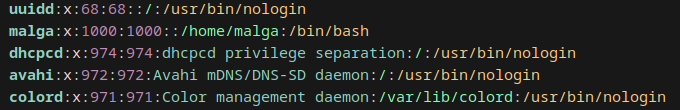
\includegraphics[width=0.7\textwidth]{images/pwd_file.png}
  \end{mdframed}
\end{frame}

\begin{frame}
\frametitle{Honeywords: Honeychecker}
\subsection{Honeychecker}
	\begin{itemize}
		\item seperate hardened system
		\item store index of the correct passwords
		\item alarms system if password file is breached
	\end{itemize}

Two functions:
\[Set(i,j)\]
\[Check(i,j)\]
\end{frame}

\begin{frame}[fragile, plain]
\frametitle{Honeywords: Login Procedure}
  \begin{figure}
    \centering
    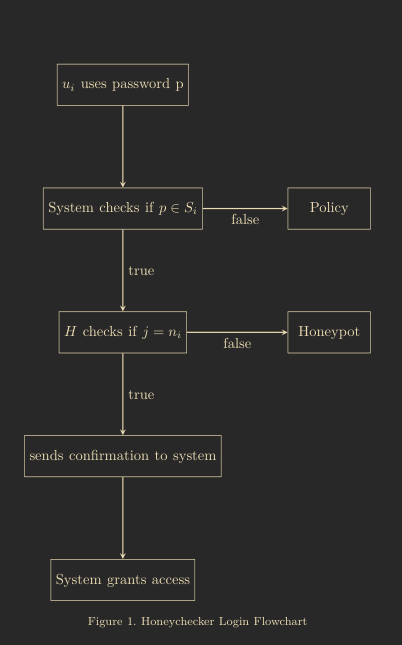
\includegraphics[height=0.8\textheight]{images/login.png}
    \caption{Honeychecker Login Flowchart}
    \label{fig:Figure1}
  \end{figure}
\end{frame}

\begin{frame}
\frametitle{PAPKE}
\section{PAPKE}
	\begin{itemize}
	\item Gen(pwd) -> \((sk, apk)\)
	\item Enc(apk, pwd) -> \(c = (c_1, c_2, c_3)\)
	\item Dec(c, pwd) -> \(k\)
	\end{itemize}
\end{frame}

\begin{frame}
\frametitle{PAPKE}
Decryption
\begin{itemize}
	\item \(k \leftarrow \{1,0\}^l\)
	\item \(y_2 \leftarrow Y_2 \cdot H_0(pwd)^{-1}\)
	\item \(R \leftarrow G\)
	\item \((r_1, r_2) \leftarrow H_1(R, y_1, y_2, k)\)
	\item \(c_1 \leftarrow g_1^{r_1} g_2^{r_2}\)
	\item \(c_2 \leftarrow y_1^{r_1} y_2^{r_2} \cdot R\)
	\item \(c_3 \leftarrow H_2(R) \oplus k\)
	\item \(c = (c_1, c_2, c_3)\)
\end{itemize}
\end{frame}

\begin{frame}
\frametitle{SweetPAKE}
\section{SweetPAKE}
\begin{itemize}
	\item Gen(pwd) -> (apk, sk)
	\item Enc(pwd, apk) -> C
	\item Dec(sk, C) -> key
	\item Retrieve\_key(i) -> key
\end{itemize}
\end{frame}

\begin{frame}
\frametitle{SweetPAKE}
Encryption part: 
\begin{itemize}
\item \(k \leftarrow \{0,1\}^*\)
\item \(K = PRF(k, (id_a, apk))\)
\item \(C[i] \leftarrow Enc(pwd, apk, K[i])\)
\item \((C', pmap) \leftarrow RP(C)\)
\end{itemize}
\end{frame}

\begin{frame}
\frametitle{Application: Requirements}
\section{Application}
\subsection{Requirements}
\begin{itemize}
\item Implementation of BeePAKE
\item Implementation of Honeywords generation algorithms
\item will work on Python 2 or higher
\end{itemize}
	Perfomance: Let \(k\) be the number of sugarwords in a password file
	Let \(T\) be the acceptable time required to share a key using the
	protocol:
	\[T = 25\% \cdot k\]
\end{frame}

\begin{frame}
\frametitle{Application: Requirements Template}
The function generate() should use the following template:
\begin{itemize}
	\item Description: First step of the BeePAKE protocol
	\item Parameter: No parameters
	\item Pre-condition: Protocol was started
	\item Post-condition: Generates a secret key, and a public key and returns the outbound message which will be sent
	\item Trigger: A party requests key-sharing with a server
\end{itemize}
\end{frame}

\begin{frame}
Repository named python-spake2 of warner in GitHub was used as base. 
\frametitle{Application: Design file structure}
\subsection{Design}

\begin{itemize}
	\item honeyword\_generation (directory)
	\begin{itemize}
		\item gen.py (python file)
		\item c\_pws (text file)
	\end{itemize}

	\item sweet\_pake (directory)
	\begin{itemize}
		\item file\_operation.py (python file)
		\item groups.py (python file)
		\item \_\_init\_\_.py (python file)
		\item six.py (python file)
		\item sweet\_pake.py (python file)
		\item util.py (python file)
	\end{itemize}
	\item client\_sweetPake.py (python file)
	\item pw\_file (text file)
\end{itemize}
\end{frame}

\begin{frame}
\frametitle{Application: Design data structures}
The data structures of both classes SweetPAKE\_Client and SweetPAKE\_Server:
\begin{itemize}
	\item password is the shared key stored as a byte object 
	\item ida and idb being the ids of the sides which are communicating
		with each other stored as byte object
	\item params is the integer group being used as the object of the \_Params class
	\item entropy\_f the entropy used and stored as byte object
\end{itemize}

Additional data\_structure of SweetPAKE\_Server:
\begin{itemize} 
 	\item database which is an associative array with all passwords as
			values and the usernames as values
\end{itemize}

\end{frame}

\begin{frame}[fragile]
\frametitle{Application: Production}
\subsection{Production}
Honeywords Generation Method, Chaffing-by-digits
\begin{lstlisting}[language=Python]
def gen_chaff_digits(p, k):
    positions = []
    i = 0

    sugarwords = []

    for c in p:
        if c.isdigit():
            positions.append(i)
        i += 1

    sys_random = random.SystemRandom()
    for n in range(k):
        sugarwords.append(p)
        for x in positions:
            rand = sys_random.randint(0, 9)
            sugarwords[n] = sugarwords[n][:x] 
	    	   + str(rand) 
		   + sugarwords[n][x+1:]

    sugarwords.append(p)
    return sugarwords
\end{lstlisting}
\end{frame}

\begin{frame}[fragile]
\frametitle{Application: Production}
\begin{lstlisting}[language=Python]
    def gen(self):
        #gen function
        group = self.params.group
        self.random_exponent = group.random_exponent(self.entropy_f)
        self.y1_elem = group.Base1.exp(self.random_exponent)
        self.y2_elem = group.Base2.exp(self.random_exponent)
        Y2_elem = self.y2_elem.elementmult(group.password_to_hash(self.pw))

        #self.outbound_message = (self.y1+self.Y2) <-- apk
        y1_bytes = self.y1_elem.to_bytes()
        Y2_bytes = Y2_elem.to_bytes()
        self.outbound_message =  y1_bytes + Y2_bytes

        username_size = len(self.username).to_bytes()

        outbound_id_and_message = self.side + username_size + self.username + self.outbound_message

        return outbound_id_and_message
\end{lstlisting}
\end{frame}

\begin{frame}[fragile]
\frametitle{Conclusion}
\section{Conclusion}
	Question: How to detect if a password file is in possession of
	intruders and at the same Does time prevent phishing attacks?
\begin{itemize}
	\item SweetPAKE is a good answer
	\item combines both strength of Honeywords and PAKE
\end{itemize}

Possible Technical Improvements:
\begin{itemize}
	\item Integration of honeychecker
	\item Improved benchmark system
	\item Unit tests
	\item Improved comments
	\item Refractor according to one style guide
	\item Include MAC authentication
	\item Improve Error Handling
\end{itemize}
\end{frame}

\begin{frame}[fragile]
\begin{center}
    \textbf{Thank you for your attention!}\\
\end{center}
\end{frame}

\end{document}
